% TikZ Figure: Recall-Throughput and Memory-Recall Trade-off Plots
% Uses strictly audited empirical values from phase_6_4_external_comparisons.json and phase_6_4_fresh_precision_memory.json
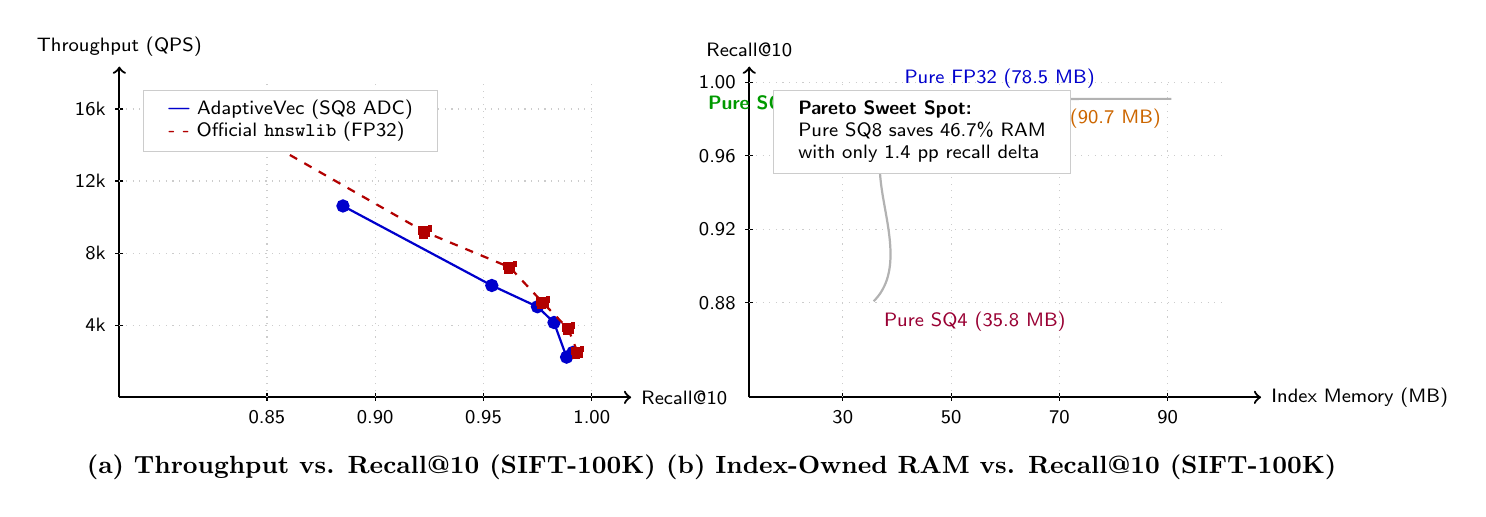
\begin{tikzpicture}[font=\sffamily\scriptsize]

% Subplot A: Recall@10 vs QPS on SIFT-100K
\begin{scope}[xshift=0cm, yshift=0cm]
    \draw[->, thick] (0,0) -- (6.5,0) node[right] {Recall@10};
    \draw[->, thick] (0,0) -- (0,4.2) node[above] {Throughput (QPS)};

    % Grid and tick marks
    % X: 0.80 to 1.00 -> map 0.80 to 0.5cm, 1.00 to 6.0cm (scale: 1 unit recall = 27.5 cm)
    % x_coord(r) = (r - 0.80) * 27.5 + 0.5
    % Y: 0 to 18,000 QPS -> map 0 to 0cm, 18,000 to 4.0cm (scale: 1 QPS = 4.0 / 18000 cm = 0.000222 cm)
    % y_coord(q) = q * 0.000222

    \foreach \r/\lbl in {0.85/0.85, 0.90/0.90, 0.95/0.95, 1.00/1.00} {
        \draw ({(\r - 0.80) * 27.5 + 0.5}, 0.05) -- ({(\r - 0.80) * 27.5 + 0.5}, -0.05) node[below] {\lbl};
        \draw[dotted, gray!40] ({(\r - 0.80) * 27.5 + 0.5}, 0) -- ({(\r - 0.80) * 27.5 + 0.5}, 4.0);
    }
    \foreach \q/\lbl in {4000/4k, 8000/8k, 12000/12k, 16000/16k} {
        \draw (0.05, {\q * 0.000222}) -- (-0.05, {\q * 0.000222}) node[left] {\lbl};
        \draw[dotted, gray!40] (0, {\q * 0.000222}) -- (6.0, {\q * 0.000222});
    }

    % AdaptiveVec Points:
    % (0.8852, 10938) -> (2.84, 2.43)
    % (0.9540, 6396)  -> (4.73, 1.42)
    % (0.9750, 5203)  -> (5.31, 1.15)
    % (0.9826, 4284)  -> (5.52, 0.95)
    % (0.9884, 2303)  -> (5.68, 0.51)
    % (0.9914, 2547)  -> (5.76, 0.57)
    \draw[thick, color=blue!80!black, mark=*] plot coordinates {
        (2.84, 2.43)
        (4.73, 1.42)
        (5.31, 1.15)
        (5.52, 0.95)
        (5.68, 0.51)
        (5.76, 0.57)
    };

    % hnswlib Points:
    % (0.8274, 16202) -> (1.25, 3.60)
    % (0.9228, 9455)  -> (3.88, 2.10)
    % (0.9622, 7450)  -> (4.96, 1.65)
    % (0.9774, 5420)  -> (5.38, 1.20)
    % (0.9892, 3931)  -> (5.70, 0.87)
    % (0.9934, 2586)  -> (5.82, 0.57)
    \draw[thick, dashed, color=red!70!black, mark=square*] plot coordinates {
        (1.25, 3.60)
        (3.88, 2.10)
        (4.96, 1.65)
        (5.38, 1.20)
        (5.70, 0.87)
        (5.82, 0.57)
    };

    \node[anchor=north west, fill=white, draw=gray!40, inner sep=3pt] at (0.3, 3.9) {
        \begin{tabular}{l}
        \textcolor{blue!80!black}{\textbf{---}} AdaptiveVec (SQ8 ADC) \\
        \textcolor{red!70!black}{\textbf{- -}} Official \texttt{hnswlib} (FP32)
        \end{tabular}
    };
    \node[below, font=\bfseries\small] at (3.2, -0.6) {(a) Throughput vs. Recall@10 (SIFT-100K)};
\end{scope}

% Subplot B: Memory vs Recall on SIFT-100K
\begin{scope}[xshift=8.0cm, yshift=0cm]
    \draw[->, thick] (0,0) -- (6.5,0) node[right] {Index Memory (MB)};
    \draw[->, thick] (0,0) -- (0,4.2) node[above] {Recall@10};

    % X: 20 to 100 MB -> map 20 to 0.5cm, 100 to 6.0cm (scale: 1 MB = 5.5 / 80 = 0.06875 cm)
    % x_coord(m) = (m - 20) * 0.06875 + 0.5
    % Y: 0.85 to 1.00 -> map 0.85 to 0.5cm, 1.00 to 4.0cm (scale: 1 unit = 3.5 / 0.15 = 23.33 cm)
    % y_coord(r) = (r - 0.85) * 23.33 + 0.5

    \foreach \m/\lbl in {30/30, 50/50, 70/70, 90/90} {
        \draw ({(\m - 20) * 0.06875 + 0.5}, 0.05) -- ({(\m - 20) * 0.06875 + 0.5}, -0.05) node[below] {\lbl};
        \draw[dotted, gray!40] ({(\m - 20) * 0.06875 + 0.5}, 0) -- ({(\m - 20) * 0.06875 + 0.5}, 4.0);
    }
    \foreach \r/\lbl in {0.88/0.88, 0.92/0.92, 0.96/0.96, 1.00/1.00} {
        \draw (0.05, {(\r - 0.85) * 23.33 + 0.5}) -- (-0.05, {(\r - 0.85) * 23.33 + 0.5}) node[left] {\lbl};
        \draw[dotted, gray!40] (0, {(\r - 0.85) * 23.33 + 0.5}) -- (6.0, {(\r - 0.85) * 23.33 + 0.5});
    }

    % Data Points:
    % SQ4: (35.75 MB, 0.8810) -> (1.58, 1.22)
    % SQ8: (41.85 MB, 0.9770) -> (2.00, 3.46)
    % FP32: (78.47 MB, 0.9910) -> (4.52, 3.79)
    % Re-rank: (90.68 MB, 0.9910) -> (5.36, 3.79)

    \draw[thick, purple!80!black, mark=triangle*] (1.58, 1.22) node[below right] {Pure SQ4 (35.8 MB)};
    \draw[thick, green!60!black, mark=*] (2.00, 3.46) node[above left] {\textbf{Pure SQ8 (41.9 MB)}};
    \draw[thick, blue!80!black, mark=square*] (4.52, 3.79) node[above left] {Pure FP32 (78.5 MB)};
    \draw[thick, orange!80!black, mark=diamond*] (5.36, 3.79) node[below left] {FP32 Rerank (90.7 MB)};

    % Trend Curve
    \draw[thick, gray!60, -] (1.58, 1.22) to[out=45, in=200] (2.00, 3.46) to[out=20, in=180] (4.52, 3.79) -- (5.36, 3.79);

    \node[anchor=north west, fill=white, draw=gray!40, inner sep=3pt] at (0.3, 3.9) {
        \begin{tabular}{l}
        \textbf{Pareto Sweet Spot:} \\
        Pure SQ8 saves 46.7\% RAM \\
        with only 1.4 pp recall delta
        \end{tabular}
    };
    \node[below, font=\bfseries\small] at (3.2, -0.6) {(b) Index-Owned RAM vs. Recall@10 (SIFT-100K)};
\end{scope}

\end{tikzpicture}
